% !TeX root = ../main.tex

\chapter{基于时间序列异常检测的根因分析系统设计与实现}
\label{cha:intro}
\section{问题描述}
在复杂系统中,无论是微服务还是云网络的场景,一方面,我们会得到单点的多个指标数据,也就是单个点上多条时间指标序列,而且由于可能是不同类型的点(例如微服务中的操作系统、数据库、容器、中间件以及云网络中的网关、交换机、虚拟机、物理机等),其指标的模式以及指标的个数都不相同。另一方面,复杂系统中当出现异常时异常会在系统中蔓延,在云网络中是通过服务调用的方式来传播,在云网络中则是流量收发包的方式。本文中我们认为这种点与点之间的拓扑是已知的。当在一个给定时间点发生一个大规模异常时,有可能有多个点以及多条链路发生故障,我们需要快速定位到是哪个节点最初发生故障并通过链路传播到了整个系统导致系统整体运行出现问题。

本文以2020AIops挑战赛《微服务应用系统故障发现和根因定位》进行复杂系统的根因分析系统设计与实现的工作。比赛中我们得到了所有节点包括操作系统、容器和数据库的单点信息,并且得到了不同节点之间调用服务的记录。其中所有节点及其静态拓扑图如图~\ref{fig:static_topo}所示。实际测试中,我们会得到若干个时间段,表示在这个时间段上整个系统出现了问题。需要我们找出的根因分为网络故障和节点故障,节点故障需要我们给出某个节点的某个指标,而网络故障如果在主机上需要给出指标,否则只需要定位到节点即可。具体的故障信息如表~\ref{tab:error}所示。

\begin{figure}[htbp]
    \centering
    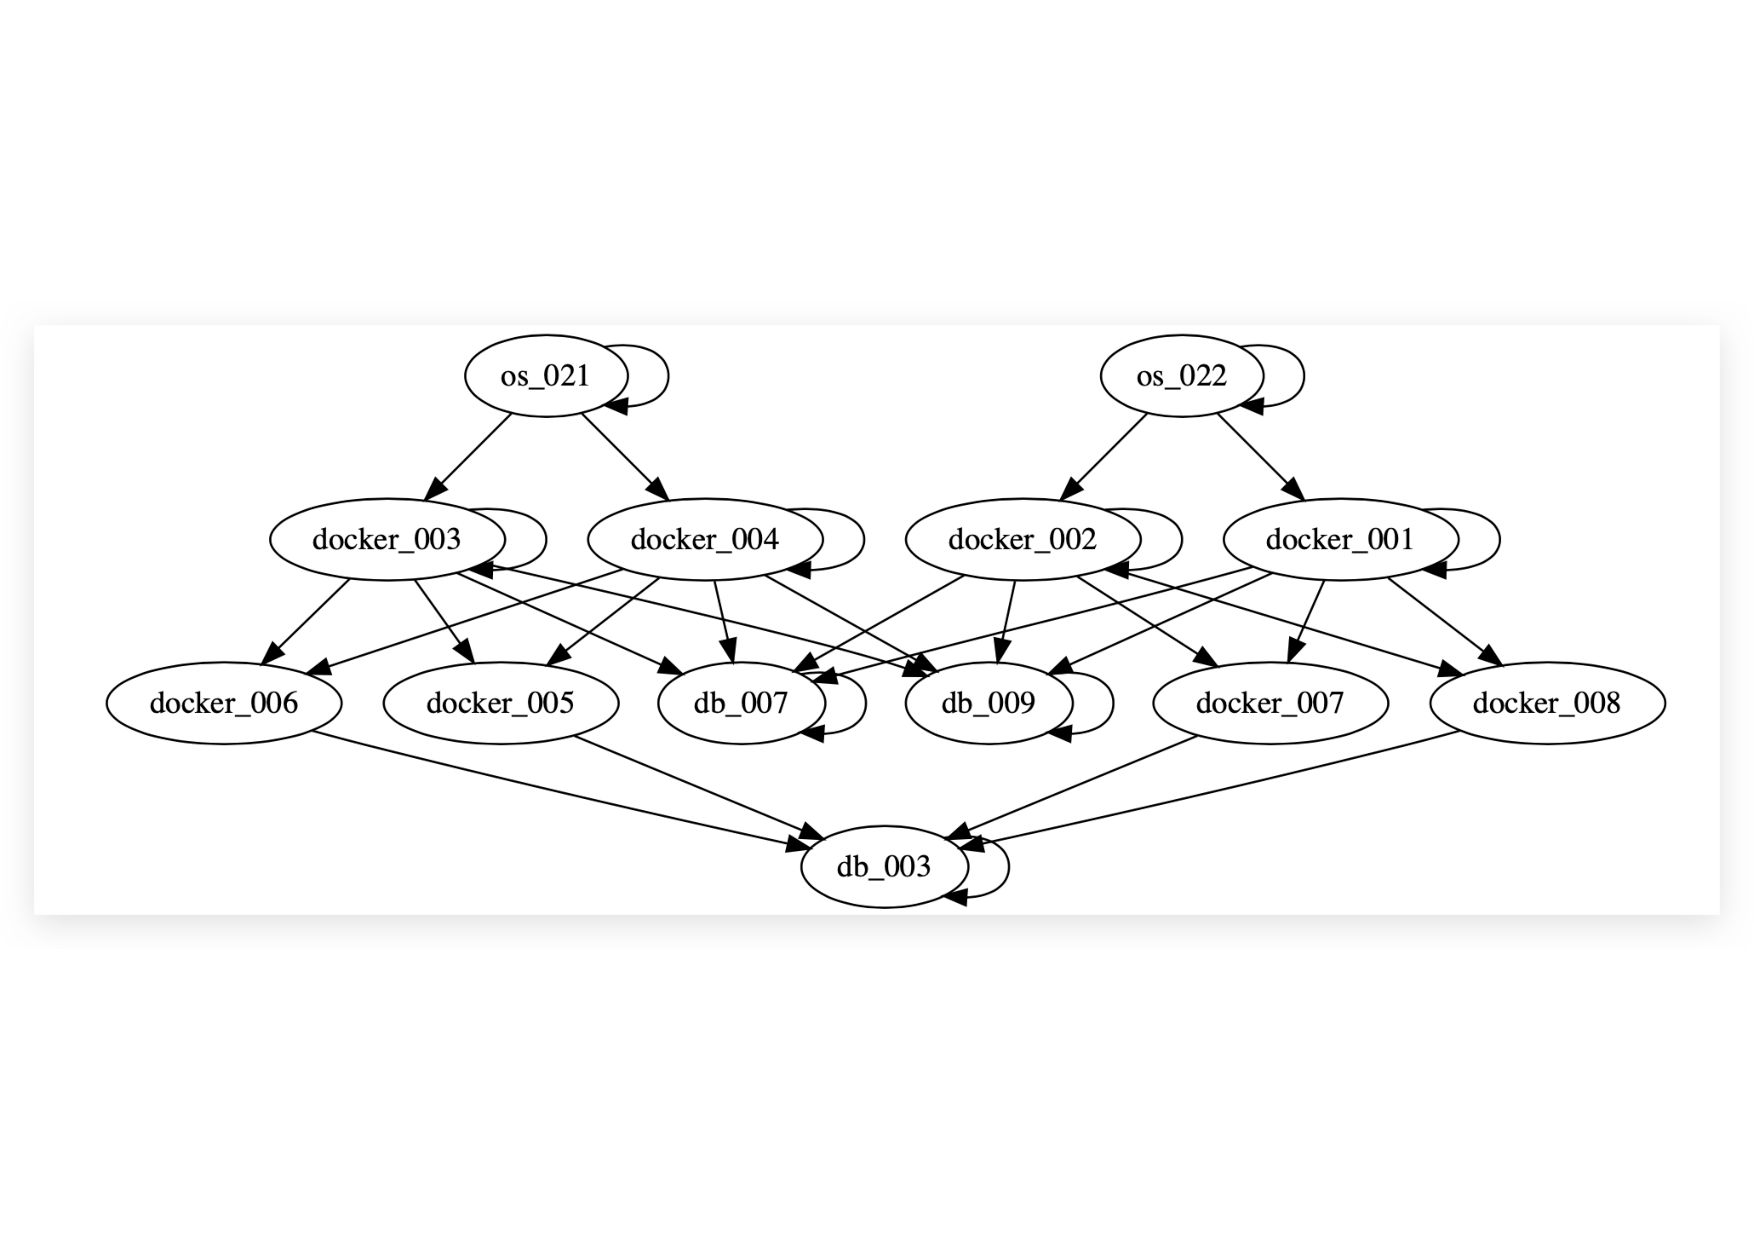
\includegraphics[width=\textwidth]{static-topo.pdf}
    \caption{静态拓扑图}
    \label{fig:static_topo}
  \end{figure}

\begin{table}
  \centering 
  \begin{tabular}{ccc}
    \toprule
    技术栈 & 场景名称 & 定位需求\\
    \midrule
    \multirow{2}{*}{数据库oracle} & 数据库关监听 & 节点指标\\
     & 数据库连接限制 & 节点指标 \\
    \multirow{3}{*}{DCOS容器} & CPU压测 & 节点指标\\
     & 网卡丢包 & 节点\\
     & 网卡延迟 & 节点\\
    \multirow{2}{*}{主机} & 网络丢包& 节点指标\\
    & 网络延迟 & 节点指标\\
    \bottomrule
  \end{tabular}
  \caption{根因类别}
  \label{tab:error}
\end{table}

\section{框架设计}
本文设计的根因分析框架如图~\ref{fig:part2-overview}所示:
\begin{figure}[htbp]
    \centering
    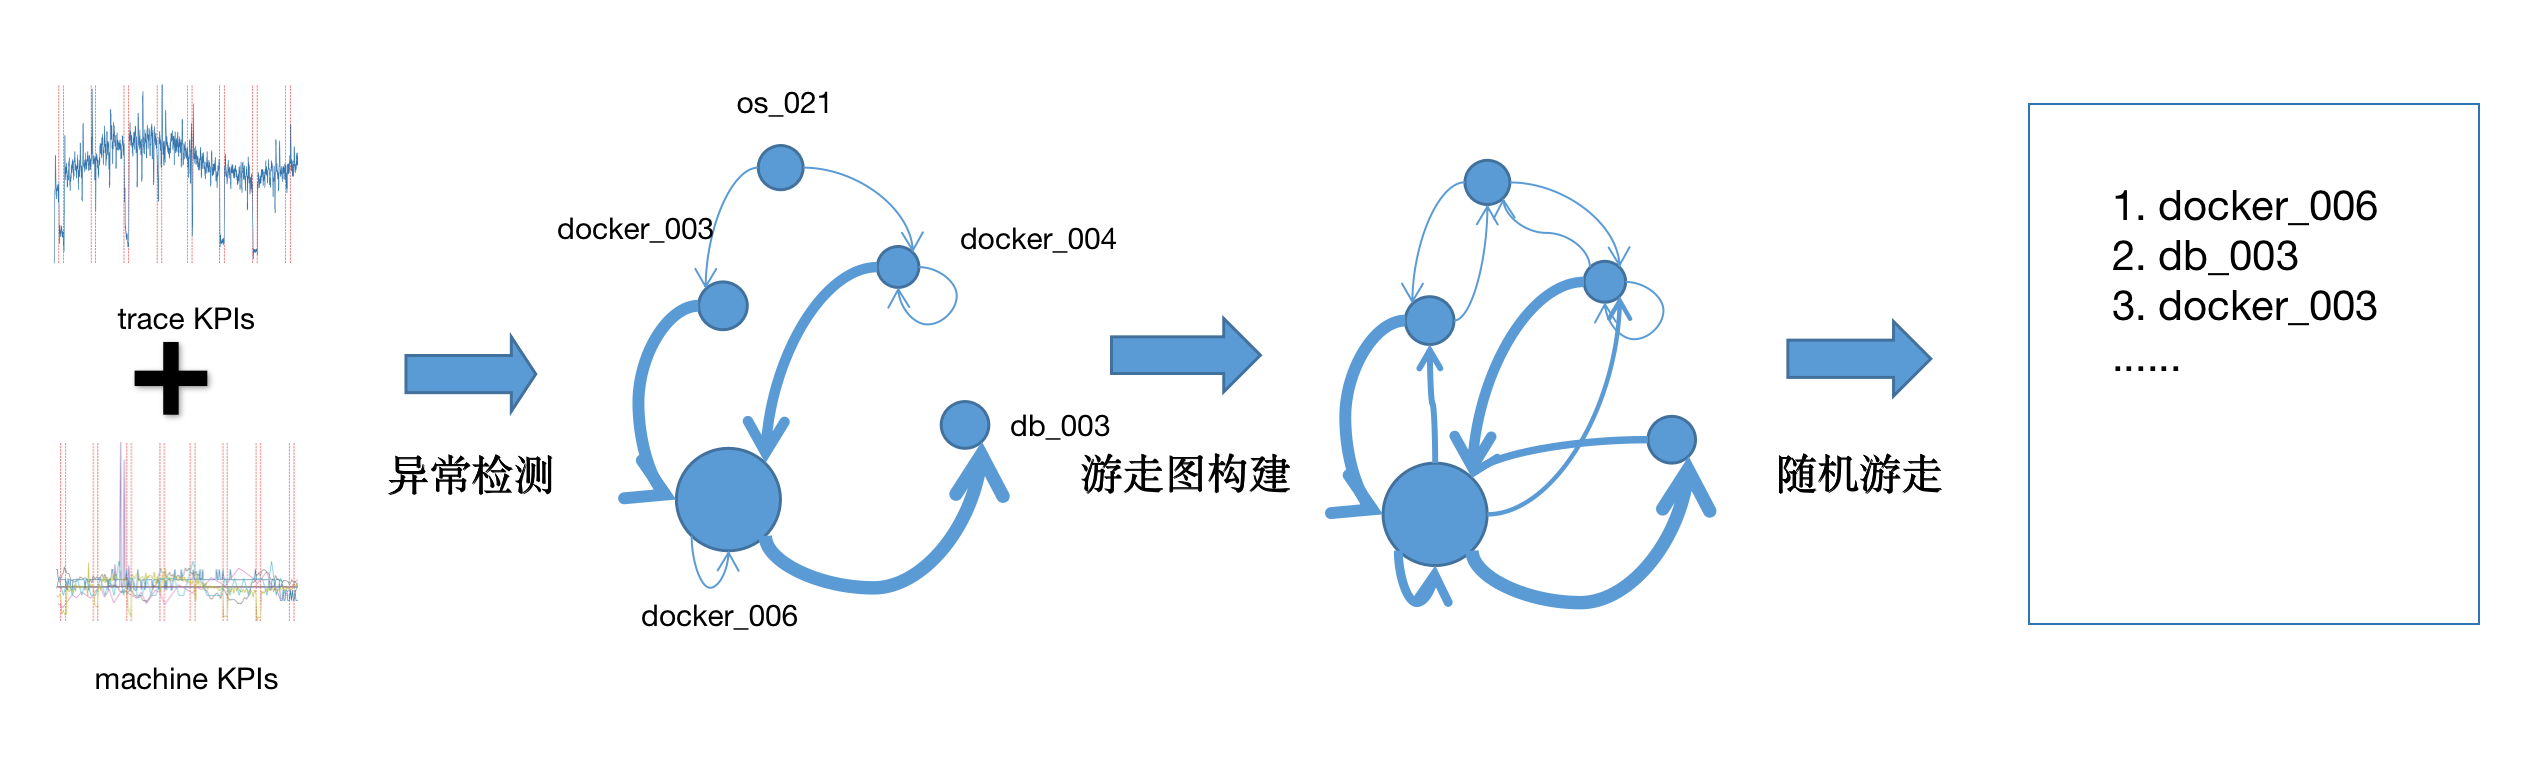
\includegraphics[width=\textwidth]{part2-overview.png}
    \caption{基于时间序列异常检测的根因分析系统框架}
    \label{fig:part2-overview}
  \end{figure}

首先我们通过预处理可以得到一系列节点上的时间序列数据和节点之间调用服务的相关指标(例如调用次数、延迟等),通过对这些时间序列数据运行异常检测算法我们得到这些曲线在某一时刻的异常分数。表现到图上的话,当一个节点的指标表现越异常,它的节点半径越大,如果一条边越异常,那么这条边就越粗。然后我们在这张图的基础上增加一些边以及修改一些边的权重,得到一张随机游走图。最后在图上运行随机游走算法来得到最有可能是根因的节点结果,然后再进一步定位到节点的指标。类似的方法理论上可以运用在云网络中进行云网络中的根因定位。接下来详细介绍各部分实现的细节。
\section{异常检测模块}
在异常检测模块,我们期望在每个故障的时刻给出每条时间序列数据的异常程度,然后再用某个聚合函数(例如max)将多条时间序列数据的分数变成单点/边的异常分数。由于单一时间序列数据得到的采样点最多只有300余个,无法使用基于深度学习的算法。因此我们需要用一些比较传统的方法,本文中我们选择了KDE\footnote{Kernel Density Estimation,核密度估计}算法,因为其计算简单、通用性强,适用于各种特性的时间序列数据,基本思路是查看故障时间点后一段时间数据的分布于前一段时间数据分布的拟合情况,两者差别越大认为该数据异常程度越高,如果基本没有差别则说明这个数据没有受到影响,其背后的节点仍在正常运作。但这个做法存在两个缺陷:一是会被偶然的突刺影响到,而这种尖刺可能是统计错误或者其他原因造成的突发状况,但不足以构成异常;二是有明显长周期性的数据问题会影响到KDE算法的正确性,因为KDE考虑到效率的原因只考虑了故障时间前后较短时间内的数据,因此如果有长周期特征的话,前后可能不符但从长远上来看是符合历史特征的,这种不应该被判断为异常。因此我们需要在采用KDE算法之前去掉明显的突刺,以及减去周期性的数据。其次,不同的时间序列数据可能具有不同的量纲和数量级。当各个数据之间差异很大的时候,直接用原数据做异常检测进行分析的话,就会突出数值较高的指标在综合分析中的作用,而削弱数值低的指标的作用。为了将所有时间序列数据的异常分数放在一起比较的结果具有可靠性,我们需要先将所有数据做归一化。因此,异常检测这部分步骤总结如下:第一步做归一化,第二步去掉尖刺数据,第三步进行周期性检测,将周期性数据从原数据中减掉,最后一步再进行KDE异常检测,输出一个异常分数。
\subsection{归一化}
目前常用的数据归一化方法主要是min-max和z-score标准化,考虑到min-max受异常值影响较大,我们采用了z-score标准化的方法。设原始数据的值为$x_i$,$mean$为原始数据的平均值,$std$为原始数据的标准差,则:
\begin{equation}
y_i = \frac{x_i-mean}{std}
\end{equation}

$y_i$为归一化后的数据,均值为0,方差为1,而且没有量纲。
\subsection{去除尖刺}
去除尖刺的目的是为了消除统计错误,也就是数据中明显不符合正常数据的凸起,而且这种凸起往往是短时间内的,例如一个时间点的数据与前后两个相邻采集点的差距都过大,我们要去除这种情况。但我们不能采用将边缘的极值去掉的方法,因为我们想要检测的异常可能就是处于边缘的极值,但是这种异常和统计错误的区别就是持续时间会相对久一些(例如5分钟以上),我们针对做以下平滑的方式:
\begin{equation}
z_i = \begin{cases} \frac{y_{i-1} + y_{i+1}}{2}, & y_i - y_{i-1} > th\ and\ y_i - y_{i+1} > th \cr \frac{y_{i-1} + y_{i+1}}{2} & y_{i-1} - y_i > th\ and\ y_{i+1} - y_i > th \cr y_i, & otherwise  \end{cases}
\end{equation}

$z_i$则为去除尖刺后的数据。
图~\ref{fig:smooth}展示了一个去除突刺的示例。其中红色标红的是出现故障的区间,如果不去除这些尖刺可能会导致在计算KDE时将尖刺统计在内而出现问题,0:45左右是真正出现故障的时间,而其他时间的波动都是正常波动,而去除尖刺之后我们很好地保留了真正的故障时段的异常,而去除了其他时刻的尖刺,保证其他时刻不会被误报。

\begin{figure}[htbp]
  \centering
  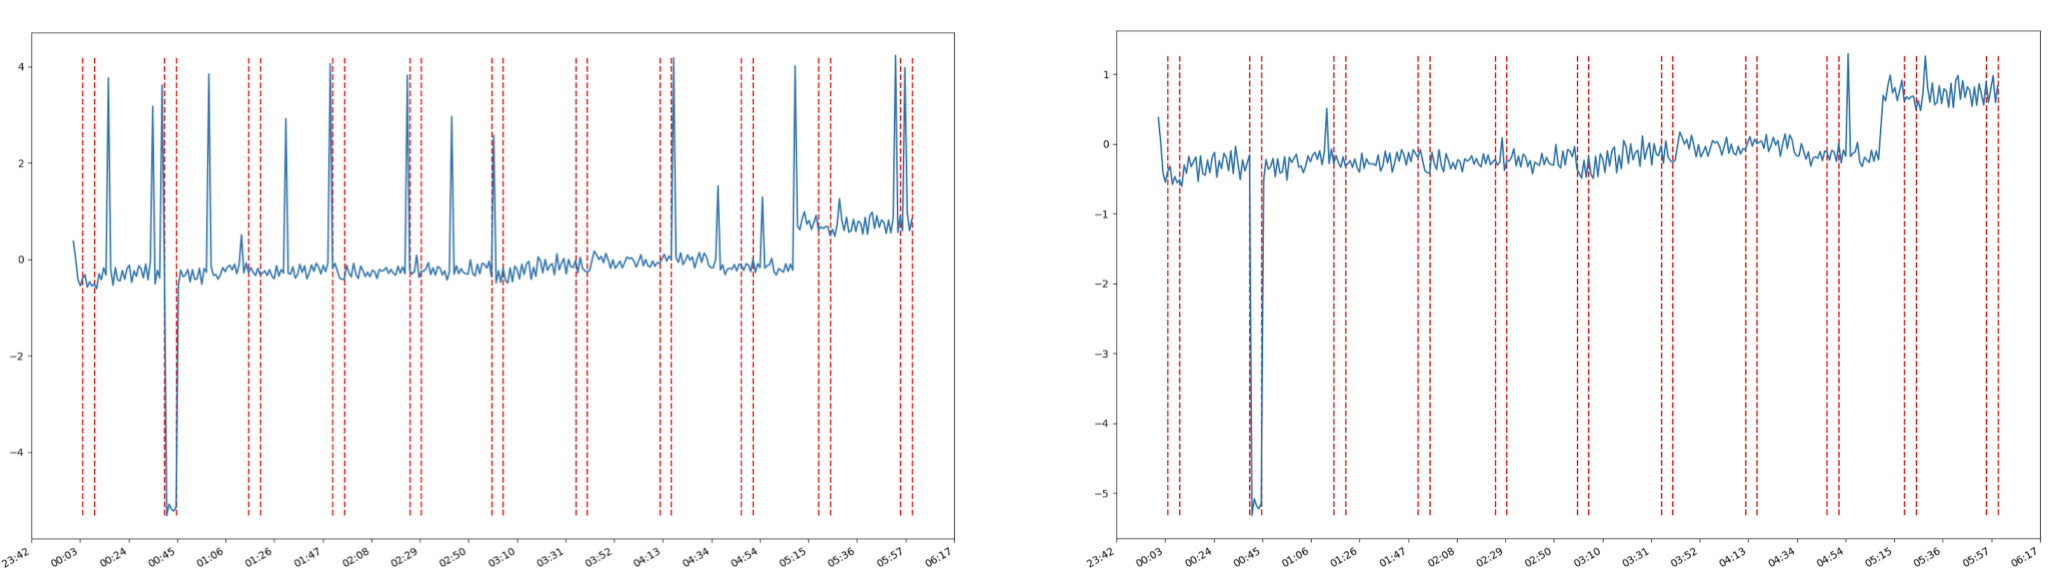
\includegraphics[width=\textwidth]{smooth.png}
  \caption{去除尖刺示例}
  \label{fig:smooth}
\end{figure}
\subsection{周期性数据去除}

在实际的时间序列数据中我们经常会遇到如~\ref{fig:period}左图所示的数据,具有很强的周期性,这样的数据完全是符合历史特征的,所以不应该被判断为异常。但如果我们用KDE算法的话,一个前提是当前数据只和周围数据相关,不会考虑到很久以前的数据,所以我们需要把周期性先给去掉。那么首先我们就要知道序列的周期是多长,这里我们用了自相关函数的方法,计算方法为:
\begin{equation}
  acf_i = \sum_{j=1}^{N-i}z_j\times z_{j+i}
\end{equation}

$acf$函数如图~\ref{fig:period}中间图所示,然后我们从画出的自相关函数图中找到第一个尖峰位置,就可以确立出函数的最小正周期是120,然后我们再统计出周期内每个位置的平均数据,并且用原数据的每个位置减去他们在周期中所处位置平均值,相当于我们将原数据分解为两部分,周期性数据和残差数据,将周期性数据减去之后得到处理好的数据如图~\ref{fig:period:right}所示,可以看到处理前的曲线有大量的起伏,如果故障时间点在中间那么无一例外这些地方都会认为是异常,而处理之后的数据尽管还留有少部分的突刺(这是因为每两个尖峰之间的距离可能不能恰好的一个周期,因此在统计时没有完全对上),但大部分时间值的分布都在0附近,说明大部分时候该曲线还是符合历史特征,不会被报为异常。
\begin{figure}[htbp]
  \begin{subfigure}[b]{0.335\textwidth}
    \begin{minipage}[t]{\linewidth}
    \centering
    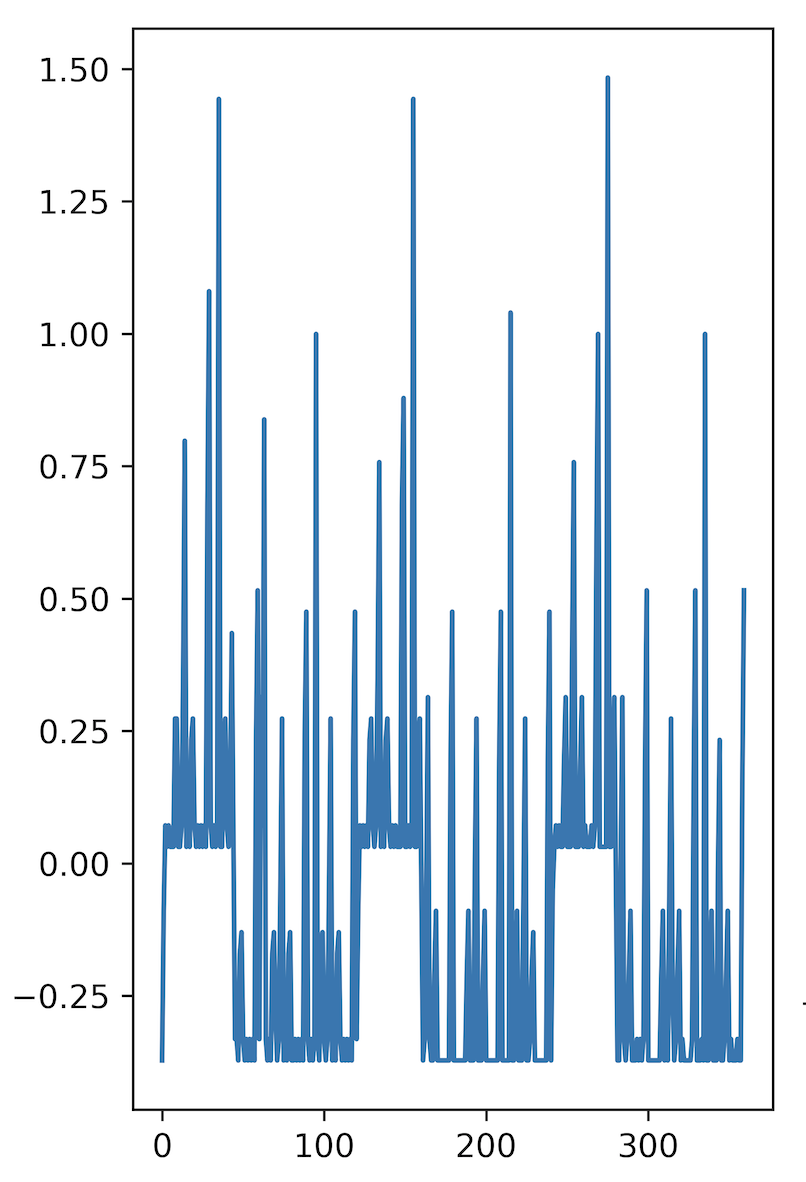
\includegraphics[width=\textwidth]{period_example_l.png}
    \caption{原始数据}
    \label{fig:period:left}
    \end{minipage}
  \end{subfigure}
  \begin{subfigure}[b]{0.325\textwidth}
    \begin{minipage}[t]{\linewidth}
    \centering
    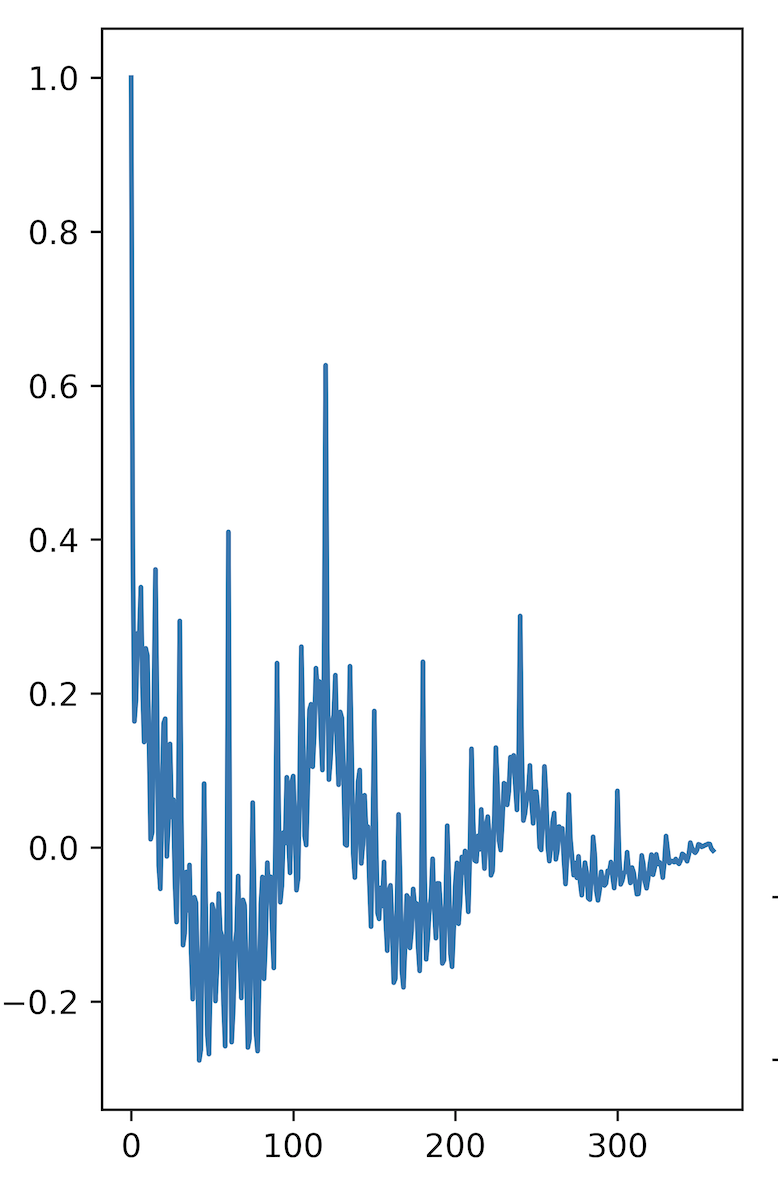
\includegraphics[width=\textwidth]{period_example_m.png}
    \caption{自相关函数}
    \label{fig:period:middle}
    \end{minipage}
  \end{subfigure}
  \begin{subfigure}[b]{0.325\textwidth}
    \begin{minipage}[t]{\linewidth}
      \centering
      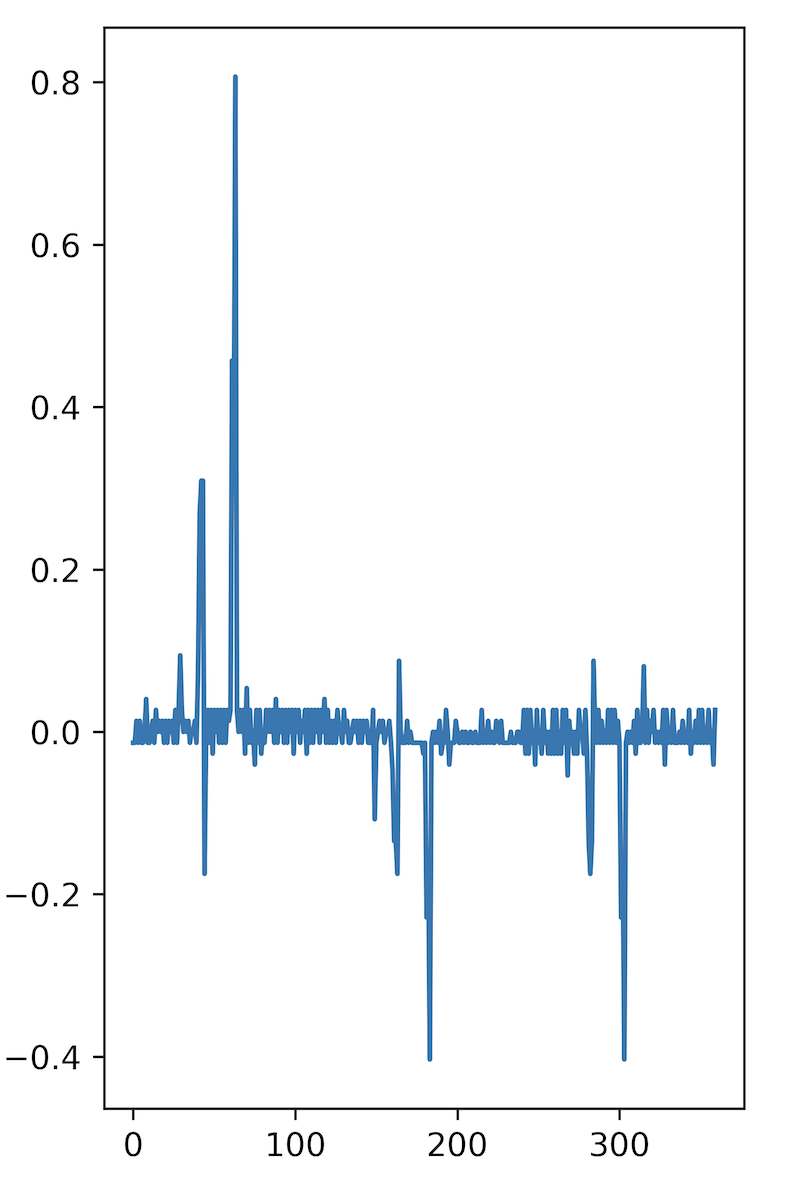
\includegraphics[width=\textwidth]{period_example_r.png}
      \caption{去除周期后的数据}
      \label{fig:period:right}
      \end{minipage}
    \end{subfigure}
    \caption{对数据去除周期化的过程}
    \label{fig:period}
\end{figure}
\subsection{KDE异常检测}
KDE是概率论中用来估计未知函数密度的非参数检验的方法之一,可以根据观察到的样本来估计随机变量的概率密度函数。
\begin{equation}
\hat{P}(x) = \frac{1}{n}\sum_{i=1}^nK(x;x_i)
\end{equation}

其中$K$是可选取的核函数,本文中我们采用了高斯核函数,$n$则是采样个数。KDE的核心思想就是对每个采样点形成一个一定带宽的核函数然后将所有采样点的核函数叠加起来作为对该数据的分布估计,本文采取的带宽为0.4。当有了密度函数之后,我们就可以用来计算新出现的数据概率了。此次竞赛中故障的持续时间总是5分钟,当给出故障时间点时,我们用前15分钟的数据来估计出一个密度函数,然后再来评估故障发生之后5分钟内数据出现的概率,概率越低说明这段时间的数据越异常,那么异常分数就越高。设之后5分钟内的数据为$x_1,x_2,\dots,x_k$,而前15分钟内用KDE得到的密度函数为$\hat{P}(x)$,则异常分数为:
\begin{equation}
  Score = \frac{1}{k}\sum_{i=1}^k\ln P(x_i)
\end{equation}

其中求均值是为了消除5分钟内不同曲线可能采样点个数不同带来的影响。
\section{根因分析模块}
在异常检测模块,我们得到了每条曲线在该时刻的异常分数,对于一个点来说,我们认为他的异常分数就是所有曲线的异常分数的最大值,对于边来说,因为有重边的存在,因此我们认为边的异常分数是所有重边的曲线分数的异常分数的平均值。由此我们可以得到如图~\ref{fig:error:example}所示的故障示例,其中点的大小代表点的异常分数的大小,而边的粗细代表边的异常分数的大小。
\begin{figure}[htbp]
  \centering
  \begin{subfigure}[b]{\textwidth}
    \begin{minipage}[t]{0.5\linewidth}
      \centering
      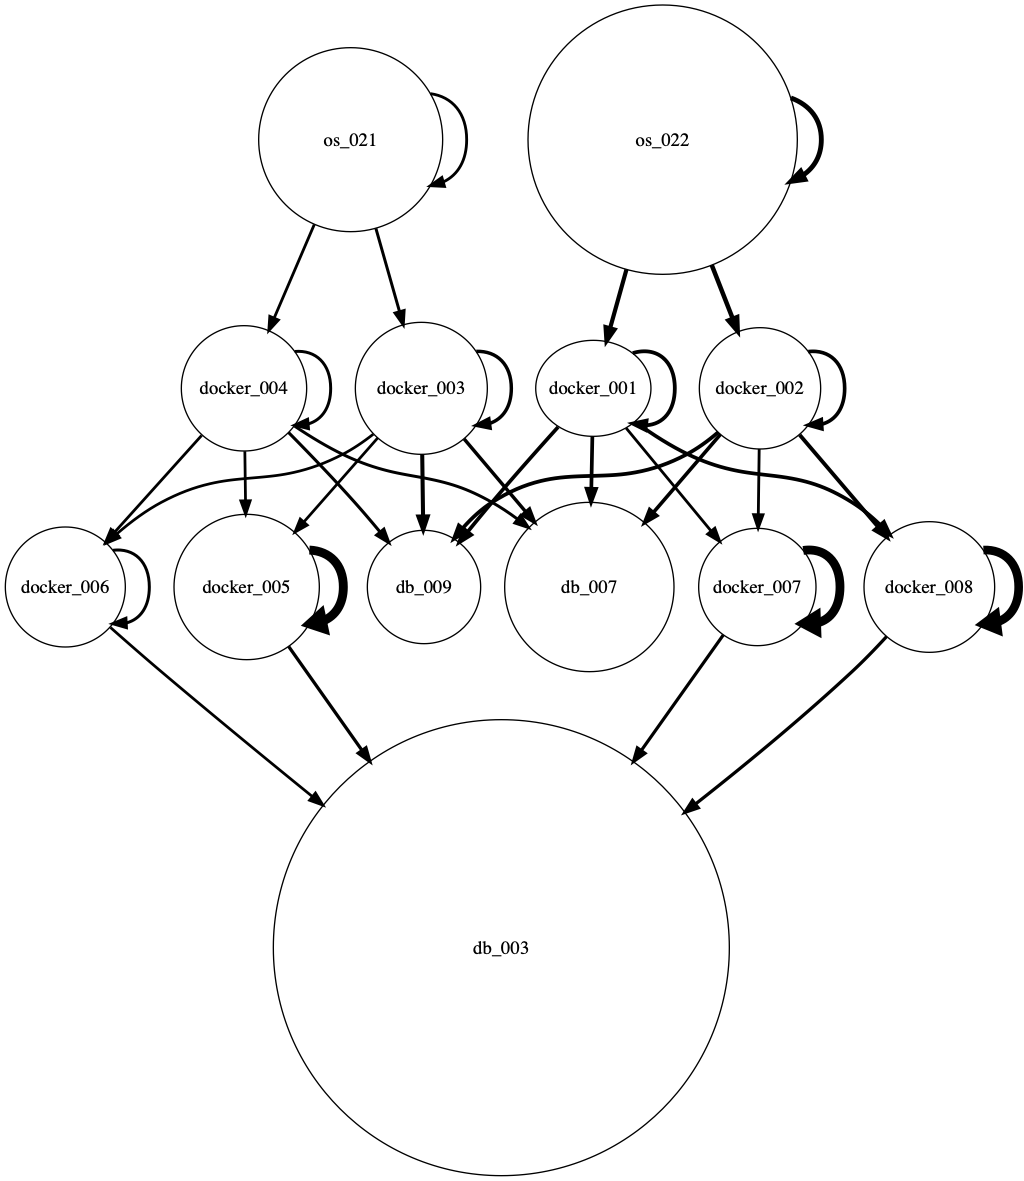
\includegraphics[width=\textwidth]{db_error.png}
      \caption{数据库关监听}
      \label{fig:error:db}
    \end{minipage}
    \begin{minipage}[t]{0.5\linewidth}
      \centering
      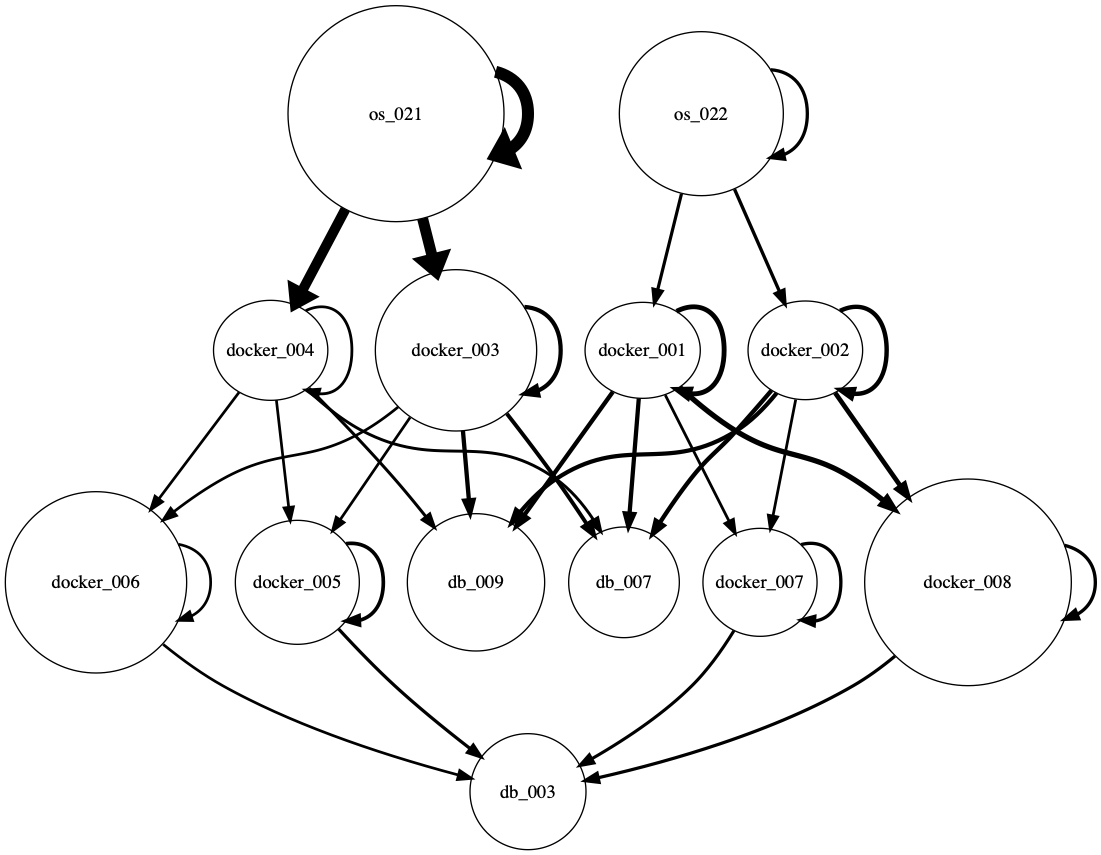
\includegraphics[width=\textwidth]{os_error.png}
      \caption{主机网络故障}
      \label{fig:error:os}
    \end{minipage}
  \end{subfigure}

  \begin{subfigure}[b]{\textwidth}
    \begin{minipage}[t]{0.5\linewidth}
      \centering
      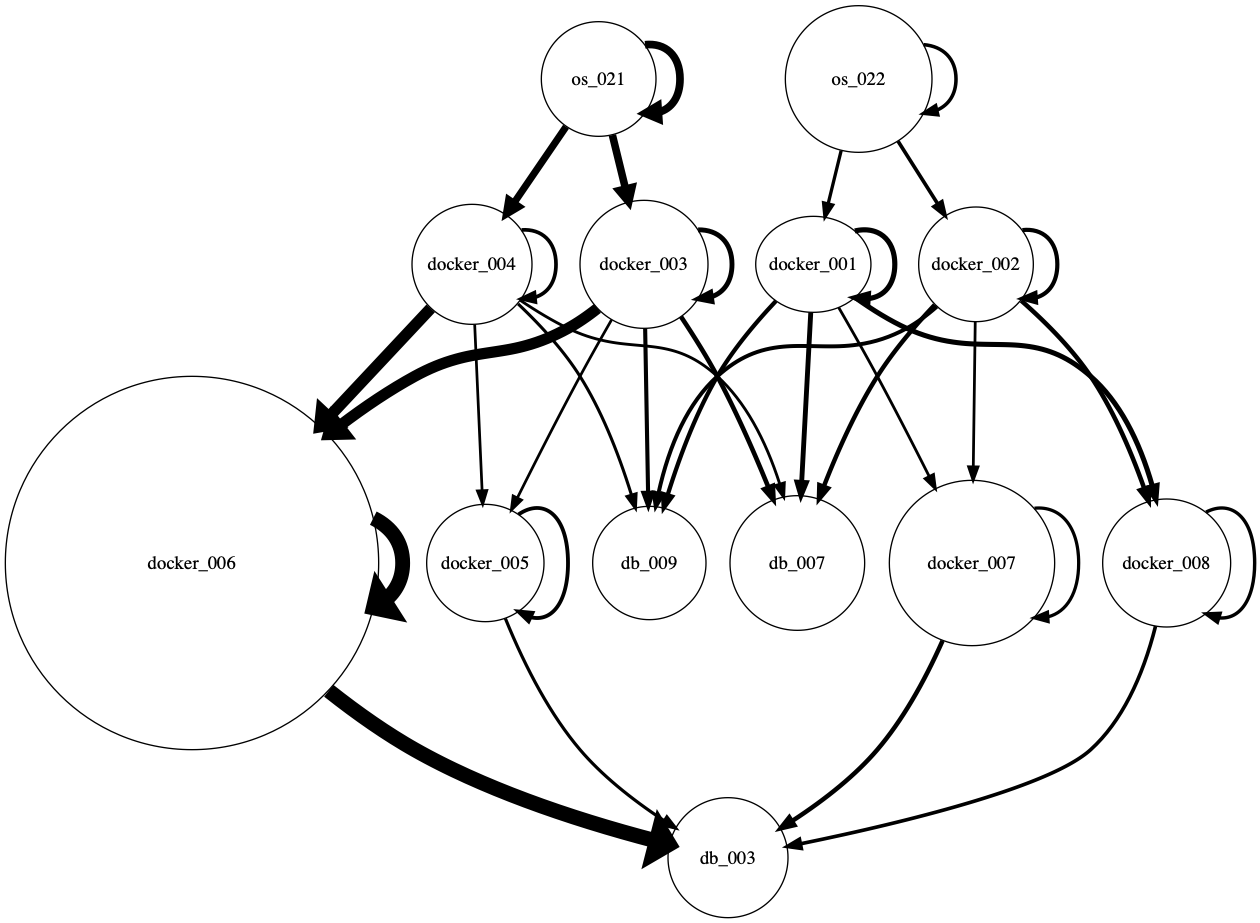
\includegraphics[width=\textwidth]{docker_cpu_error.png}
      \caption{容器cpu压测}
      \label{fig:error:db}
    \end{minipage}
    \begin{minipage}[t]{0.5\linewidth}
      \centering
      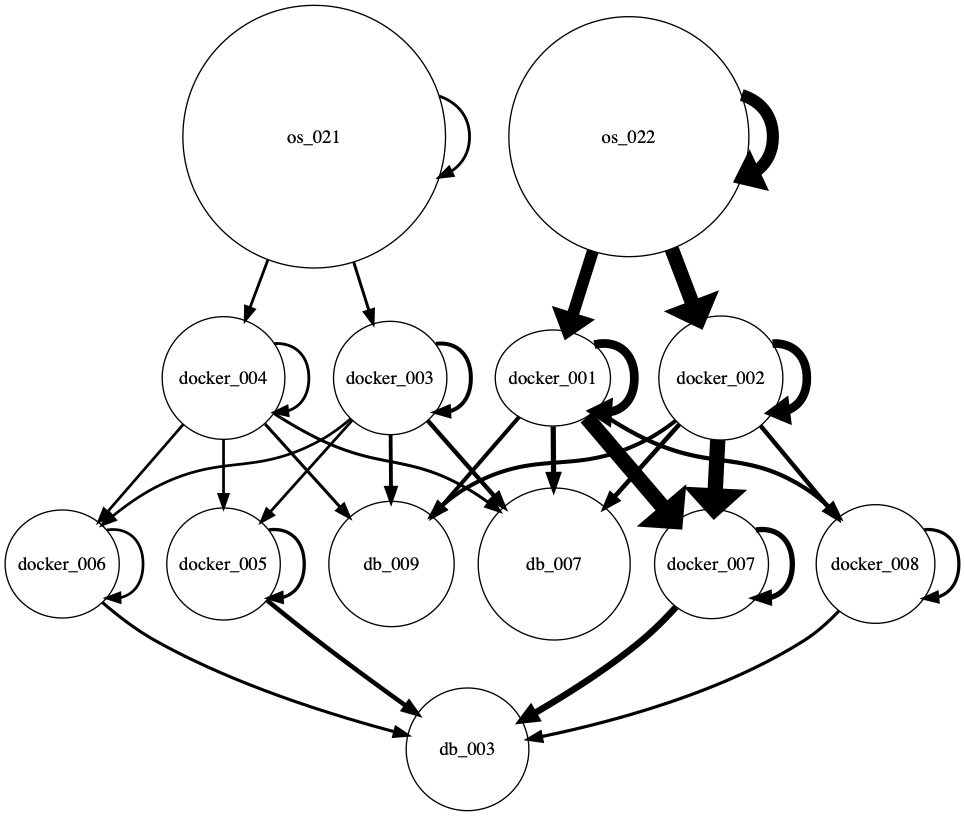
\includegraphics[width=\textwidth]{docker_network_error.png}
      \caption{容器网络故障}
      \label{fig:error:os}
    \end{minipage}
  \end{subfigure}
  \caption{AIOPS2020挑战赛中故障示例}
  \label{fig:error:example}
\end{figure}
\subsection{构建随机游走图}
我们要在原先的异常图的基础上构建随机游走图。不妨设原图$G=(V,E)$,点$i$的点权为$v_i$,边权为$w_{i,j}$,我们要在此基础上加入反向边和自环,具体方法如下:
\begin{itemize}
  \item 前向边:为了运行随机游走算法,边的方向应当代表异常传播的方向。当一个$i$调用$j$的服务调用时长发生异常时,我们认为异常是由$j$传播到$i$,因此异常传播的方向与服务调用的方向相反,也就是根因的方向与服务调用的方向相同。所以该部分保持不变;
  \item 反向边:因为随机游走具有一定的随机性,为了防止行走者走到一个较小概率是根因的节点,然后出不去,我们考虑加入反向边。该边的权值随正向边的权值增加而增加,也就是$w_{i,j} = \rho_{back} w_{j,i}$,如果$(i,j) \notin E\ and\  (j,i) \in E$;
  \item 自环:当节点自身就是根因的时候,我们需要增大其留在原位置的概率而不走到其他地方。我们观察到:当一个节点是根因时,它会影响到周围和它有关联的点,通常情况下所有调用它的服务的返回时间的都会出现异常,同时它调用其他节点的服务也会出现异常,因此我们要将这些因素也纳入考量范围。总的来说我们需要考虑三个因素,一是节点本身的异常分数,二是所有其他节点到该节点的边的异常分数的平均值,三是该节点到所有其他节点的边的异常分数的平均值,也就是$w_{i,i} = \rho_{in} in\_avg\_weight_{i} + \rho_{out} out\_avg\_weight_{j}+ \rho_{self}  v_i$。另一方面,考虑到入边是推导根因的方向,所以我们在设置超参时会保证$\rho_{in}>\rho_{out}$。
\end{itemize}

总结如下:
\begin{equation}
w_{i,j} = \begin{cases} w_{i,j}, & if\ (i,j) \in E \cr \rho_{back} w_{j,i}, &\ if\ (i,j) \notin E\ and\  (j,i) \in E \cr \rho_{in} in\_avg\_weight_{i} + \rho_{out} out\_avg\_weight_{j}+ \rho_{self}  v_i, & if\ i=j \end{cases}
\end{equation}

\subsection{随机游走}
首先我们将边权矩阵$w$标准化得到转移矩阵$\overline{w}$:
\begin{equation}
  \overline{w}_{i,j} = \frac{w_{i,j}}{\sum_jw_{i,j}}
\end{equation}

然后由于$os_{021}$和$os_{022}$是整张拓扑图的入口,因此我们以这两个点为起点,随机游走1000次,统计每个节点被经过的次数。进一步的,为了避免行者到某个不是根因的节点出不去,我们将这个过程重复10遍,消除其中的随机性带来可能的答案错误。最后按到达次数对节点进行排序。最后我们选取到达次数最多的节点,输出其节点上异常分数最高的曲线作为最终的根因。此外,是当该节点本身的异常分数比较小,且没有向下传播异常的时候,我们认为是该节点的网络故障而不是cpu故障。

\section{结果}
目前,本文提出的算法在该竞赛目前已公布的前两阶段数据中可以获得100\%的正确率。

\section{小结}
本章详细介绍了基于时间序列异常检测的根因分析系统,对节点上的时间序列数据和节点之间的服务调用相关的时间序列数据运行KDE异常检测算法得到异常分数,以此为基础构建异常传播图,在这个图上进行随机游走算法来得到每个节点的经过次数,最多的即认为是根因。所用方法投入AIOPS2020使用之后在前两阶段获得了100\%的正确率。